\section{Operacioni pojačavač}

{Operacioni pojačavac je aktivna provodnička komponenta koja
pojačava razliku potencijala na svojim ulazima. Aktivna je komponenta
zato što za svoj rad zahteva spoljašnje napajanje, čime se omogućava
da izlazni signal ima veću snagu od ulaznog signala.
Izgled operacionog pojačavača je prikazan na slici \ref{fig:opamp}.}

\begin{figure}[ht]
    \centering
    \begin{circuitikz}[american]
        \begin{scope}
            \ctikzset{tripoles/op amp/width=2.5,   % default 2.5
                    tripoles/op amp/height=2}    % default 2
            \node[op amp] (OA) at (0,0) {};
        \end{scope}
        \draw
            (OA.+) -- ++(-1,0) node[left]{$V^{+}$}
            (OA.-) -- ++(-1, 0) node[left]{$V^{-}$}
            (OA.out) -- ++(1,0) node[right]{$V_{out}$};

        \draw
            (OA.up) -- ++(0,1) node[above]{$+V_{cc}$};

        \draw
            (OA.down) -- ++(0,-1) node[below]{$-V_{cc}$};
    \end{circuitikz}
    \caption{Operacioni pojačavač}
    \label{fig:opamp}
\end{figure}

{Operacioni pojačavač ima dva naponska ulaza, jedan je invertujući $V^{-}$,
a drugi neinvertujući $V^{+}$ i jedan izlaz $V_{out}$. Takođe ima dva priključka
za napajanje $+V_{cc}$ i $-V_{cc}$. Operacioni pojačavač na svom izlazu
$V_{out}$ daje pojačanu razliku potencijala na ulazima $V^{+}$ i $V^{-}$.
Ovo je dato sledećim izrazom}

\begin{equation}
    V_{out} = A_{o} \cdot (V^{+} - V^{-}).
\end{equation}

{$A_{o}$ predstavlja pojačanje operacionog pojačavača
u otvorenoj sprezi. Njegova vrednost zavisi od karakteristika
i specifikacije konkretnog operacionog pojačavača, obično je reda veličine $10^5$ do $10^6$. Vrednosti na izlazu operacionog pojačavača su ograničene napajanjem, tako da se uvek kreću između $+V_{cc}$ i $-V_{cc}$. Iz ovog zaključka može se izvesti izraz za maksimalnu vrednost ulaza operacionog pojačavača}

\begin{equation}
    -V_{cc} \le V_{out} \le +V_{cc},
\end{equation}

{odnosno zato što je $V_{out} = A_o V_{in}$}

\begin{equation}
    \frac{-V_{cc}}{A_o} \le V_{in} \le \frac{+V_{cc}}{A_o}.
\end{equation}

{Demonstracija u \href{https://www.desmos.com/calculator/83gqbywenh}{Desmos}-u}

\pagebreak
\subsection{Karakteristike idealnog operacionog pojačavača}

{Shema idealnog operacionog pojačavača data je na slici \ref{fig:opamp_ideal}.}

\begin{figure}[ht]
    \centering
    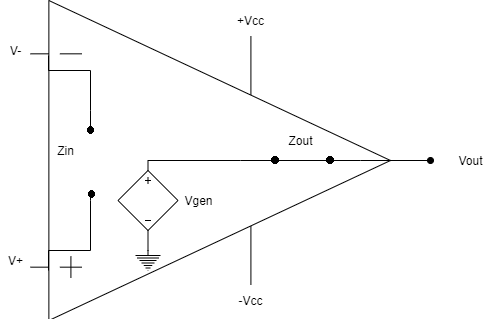
\includegraphics[width=0.6\textwidth]{opamp_ideal.png}
    \caption{Shema idealnog operacionog pojačavača.}
    \label{fig:opamp_ideal}
\end{figure}

{Na osnovu slike može se zaključiti da idealni operacioni pojačavač
ima sledeće karakteristike:}

\begin{enumerate}
    \item {$A_{o} = \infty$} - operacioni pojačavač u otvorenoj sprezi
    ima beskonačno veliko pojačanje, što znači da će i za najmanju razliku potencijala 
    na ulazu imati beskonačno veliki izlazni napon.
    \item {$Z_{in} = \infty$} - operacioni pojačavač ima beskonačno veliku ulaznu impedansu, što znači da ne teče struja kroz ulazne priključke operacionog pojačavača.
    \item {$Z_{out} = 0$} - operacioni pojačavač ima nultu ulaznu impedansu, što znači da se ponaša kao idealni naponski izvor (ne opterećuje kolo na bilo koji način).
    \item {Karakteristike rada operacionog pojačavača ne zavise od frekvencije ulaznog signala}
\end{enumerate}

{Ovakva izvedba operacionog pojačavača predstavlja samo idealizovan matematički
model i kao takav nije ga moguće realizovati u praksi. Već se on može
posmatrati kao nešto čemu inženjeri teže pri dizajniranju operacionih pojačavača.}
